\documentclass{article}
\usepackage{graphicx}
\usepackage{authblk}
\usepackage{amsmath}
\usepackage{textcomp}
\usepackage{color}
\usepackage{listings}
\lstset{language=Matlab}

\begin{document}
\title{THEORETICAL NEUROSCIENCE \\ EXERCISE 9}
\date{9. Dec 2012}
\author[1]{\c{S}eyma Bayrak\thanks{seyma.bayrak@st.ovgu.de}}
\affil[1]{\footnotesize  Otto von Guericke University of Magdeburg}
\maketitle

\section{Introduction}
\textbf{Psychophysics} is a science of measuring subjective sensory experiments in which the stimuli is controlled by the experimenter. \textbf{Signal Detection Theory - STD} applies to psychophysics and provides a graphical analaysis to clear uncertainities on it. The four key concepts is frequently used to complete the STD of an experiment: \textit{Noise, Criterion, ROC, $P_.{correct}$}.\\

Identical sensory events of stimulus result in subjective responses on the neuron. However, an isolated stimulus of noise (as in our exercise) might also lead the observer to detect the response. The first step of STD approach is to define a \textbf{decision criterion} by the observer. It means that, whenever the response of stimuli exceeds the criterion, the observer saves it as being "detected".\\

The detection of two stimuli (one can be simulated as 'noise') has four possible statistical outcomes: \textit{Hits, Misses, False Alarms, Rejections}. \textit{Hits} mean the outcome of stimuli that exceed criterion, whereas \textit{Misses} for the ones not exceeding criterion. \textit{False Alarms} represent the response of noise, which also exceed the criterion, and \textit{Rejections} stand for the response of noise which is under criterion. The more statistical approach can be defined as the probability distribution as in the equation below.\\

\begin{center}
$H \equiv P('yes'|'signal') \,\,\,\,\,\,\,\,\,\, F \equiv P('yes'|'noise')$ 
\end{center}  

The \textit{ROC} means the receiver operating characteristic. It is the plot of 'hits' against 'false' alarms for different criterion levels. ROC reveals the optimal criterion and therefore the optimal performance. The final key step of STD is defined as $P_{correct}$; it is the proportion of overall correct response against the stimuli level (e.g. light intensity). \\

Exercise 9 is provided with a function called \textbf{VisResp}, which takes an input vector \textbf{s} of size of \textbf{N}, and creates an output vector of the same size. The STD analyse of stimuli with different stimuli level (different s levels) and different criterions are explained step by step in programming assignment part.

\begin{equation*}
 r=\textbf{VisResp}(s)
\end{equation*}


\section{Programming Assignment}

\subsection{Describing the Response}

The average response $<r(s)>$ is obtained for different light levels \textit{s}, $0<s<12$. Each light level is tested \textit{N} times. Figure 1 indicates the plot of s against average response. 

\begin{center}
 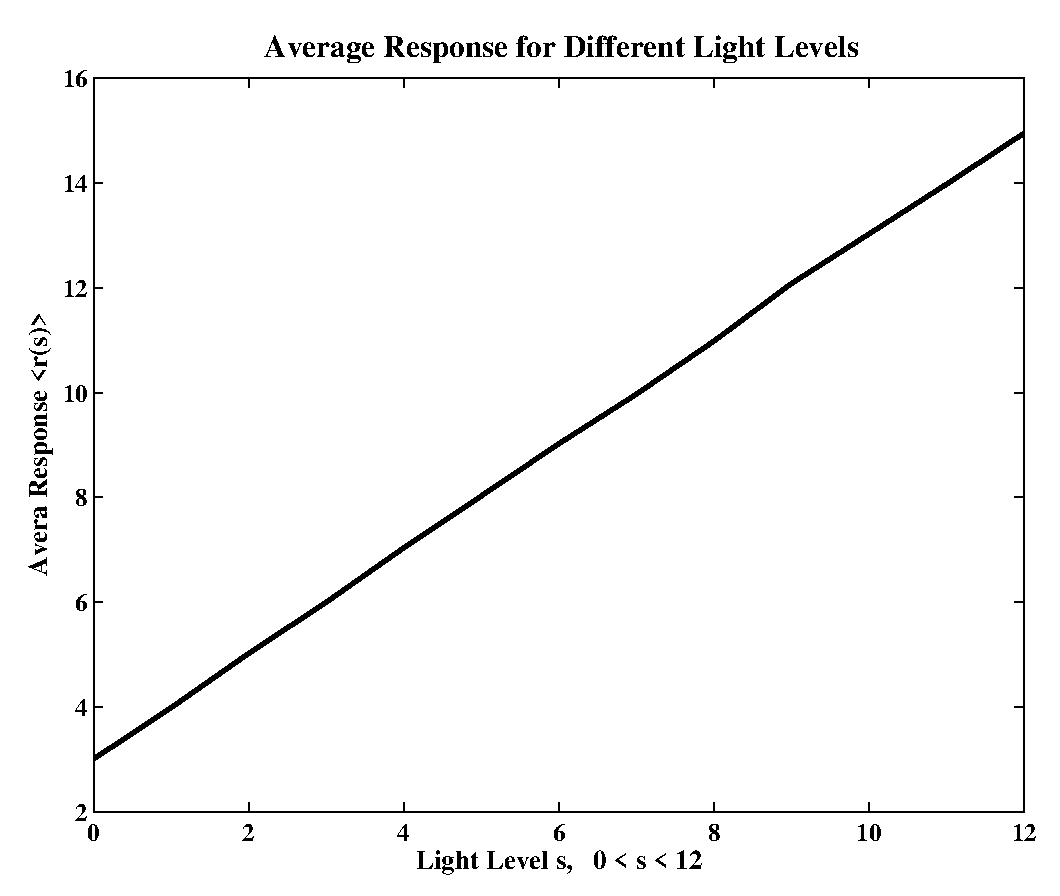
\includegraphics[width=\textwidth]{ave_resp.eps}
\begin{footnotesize} Fig. 1,$N=10000$, that means for every s value, response is computed N times and then it is averaged. 
\end{footnotesize}
\end{center} 

This time response is found for only three s values for N times, but not averaged. Instead the response distribution is computed by \textbf{hist} command on MATLAB and then converted into propability distribution. Figure 2 shows three different probability densities. 

 \begin{center}
 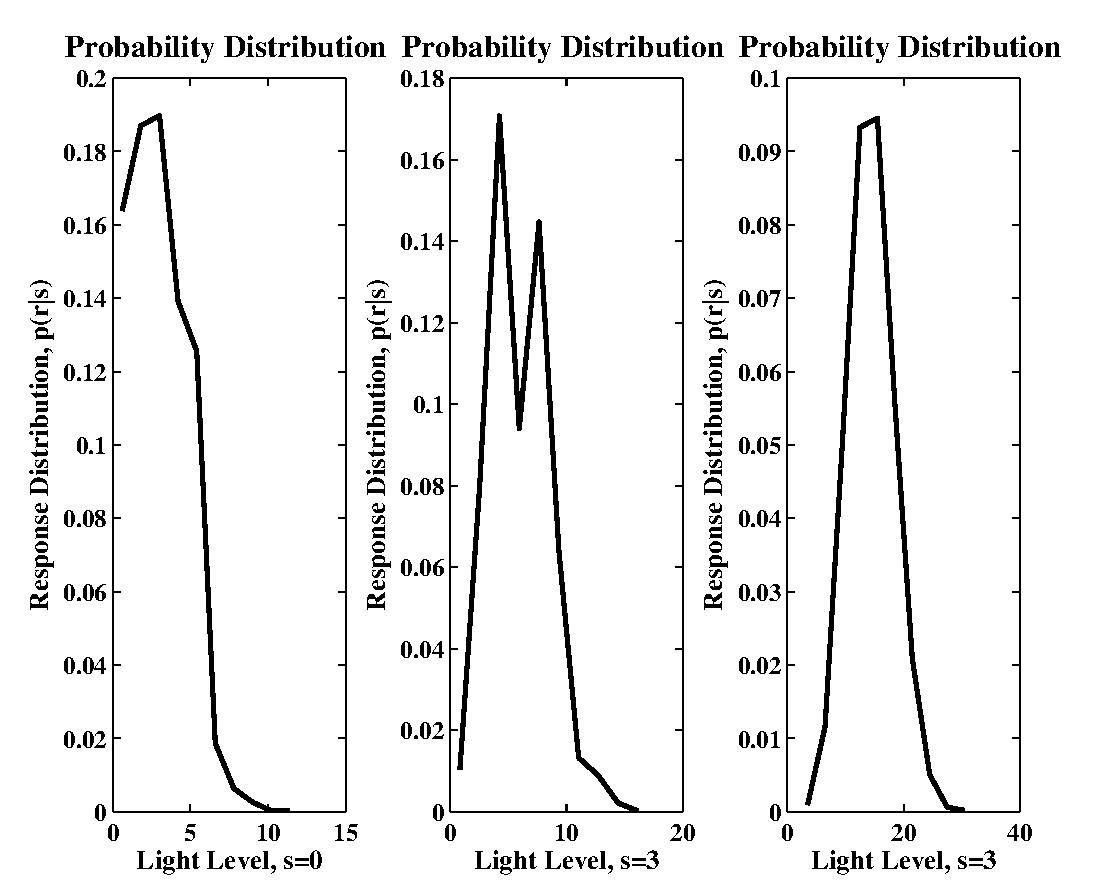
\includegraphics[width=\textwidth]{prob_dist.eps}
\begin{footnotesize} Fig. 2, probability distributions for $s=0,3,12$. 
\end{footnotesize}
\end{center}

Let us check what the area under probability densities are equal to. Graph numbers are numbered as from the left to the right on Figure 1. 

\begin{lstlisting}
Area under the probability distribution of graph number 1 is 1 ! 
Area under the probability distribution of graph number 2 is 1 ! 
Area under the probability distribution of graph number 3 is 1 !
\end{lstlisting}

\subsection{Non-optimal Decision}

This section analyzes the two types of responses; firstly the response is eliminated from the absence of light, secondly from the presence of light. Absense of light is simulated from an input vector \textbf{s} having \textit{N} terms of zero elements. Presence of light is simulated from another vector having values between 0 and 12 (inside a for loop), and it also has \textit{N} elements for each constant. As in the previous section, responses are computed each time for all values between 0 and 12.\\

We chose a criterion called $\theta$, and then make an assumption. If the elements of response vector \textbf{r} is greater than that value, the observer detects a simulation, if not, no detection. It is reasonable to get simulation from presence of light, and we call it as \textit{Hits, Right Alarms}. However, when the light is absent, it is also possible to get simulation, because \textit{r} of \textit{s=zeros} has also elements greater than $\theta$. It is called \textit{False Alarms}. The proportion of false and right alarms are shown in Figure 3. 

 \begin{center}
 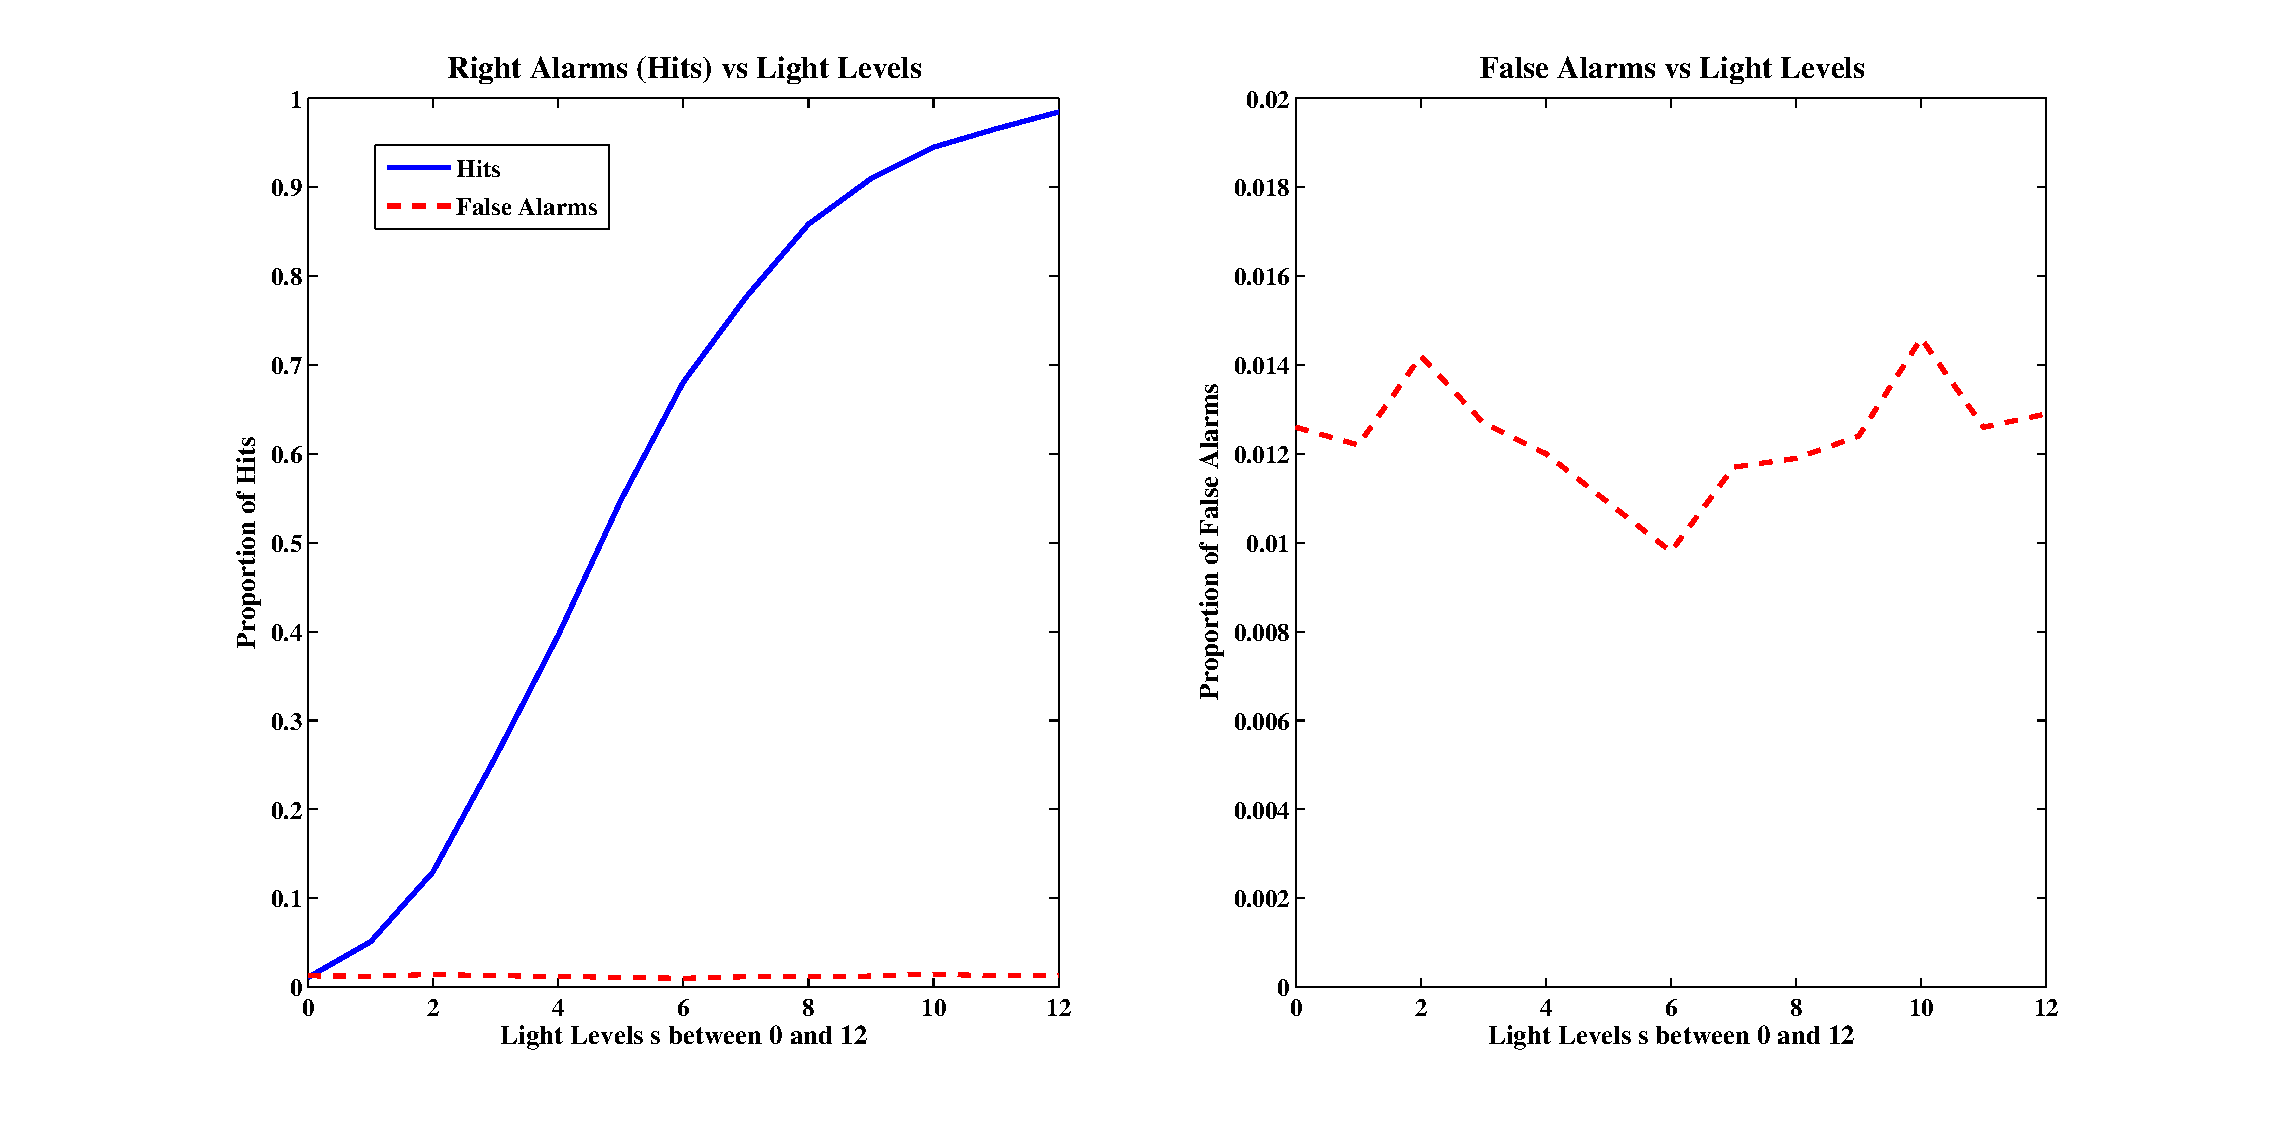
\includegraphics[width=\textwidth]{hits_false.eps}
\begin{footnotesize} Fig. 3, Left graph; proportion of hits overall s values. Here the proportion of false alarms is alce placed as dashed lines, but its range is too small, therefore it is zoomed in on the right graph.
\end{footnotesize}
\end{center}

Now a new term is defined as \textit{$P_{correct}$}. It is the proportion of right alarms \textit{Hits} overall correct responses. Figure 4 indicates $P_{correct}$ against the light level $s$. The Figure 4 is also named as \textit{neurometric function}. The equation below express how to find ${P_correct}$ value.\\

\begin{center}
$P_{correct}=\dfrac{H(\theta)+1-F(\theta)}{2}$
\end{center}

\subsection{Optimal Decision}


$\theta$ is chosen between 0 and 30. For each value of $\theta$, proportion of hits \textit{H($\theta$)} and proportion of false alarms \textit{F($\theta$)} is computed. This is done for each \textit{s} light levels between 0 and 12 as in the previous section. The plot of $H(\theta)$ versus $F(\theta)$ is called as \textit{ROC} curve. ROC means "receiver operating characteristic" for each light level \textit{s} and it is independent of any particular choice of $\theta$. Additionally, the proportionality correct \textit{$P_{correct}$} is calculated from the area under ROC curve. \\


 \begin{center}
 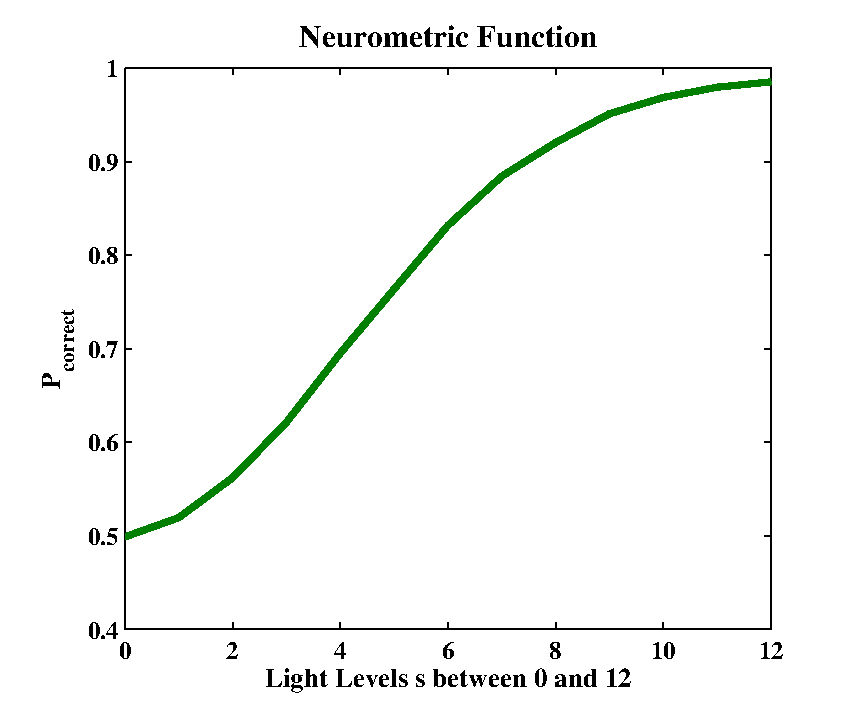
\includegraphics[width=\textwidth]{p_correct.eps}
\begin{footnotesize} Fig. 4, proportion of correct responses of overall responses against s values. 
\end{footnotesize}
\end{center} 


\begin{center}
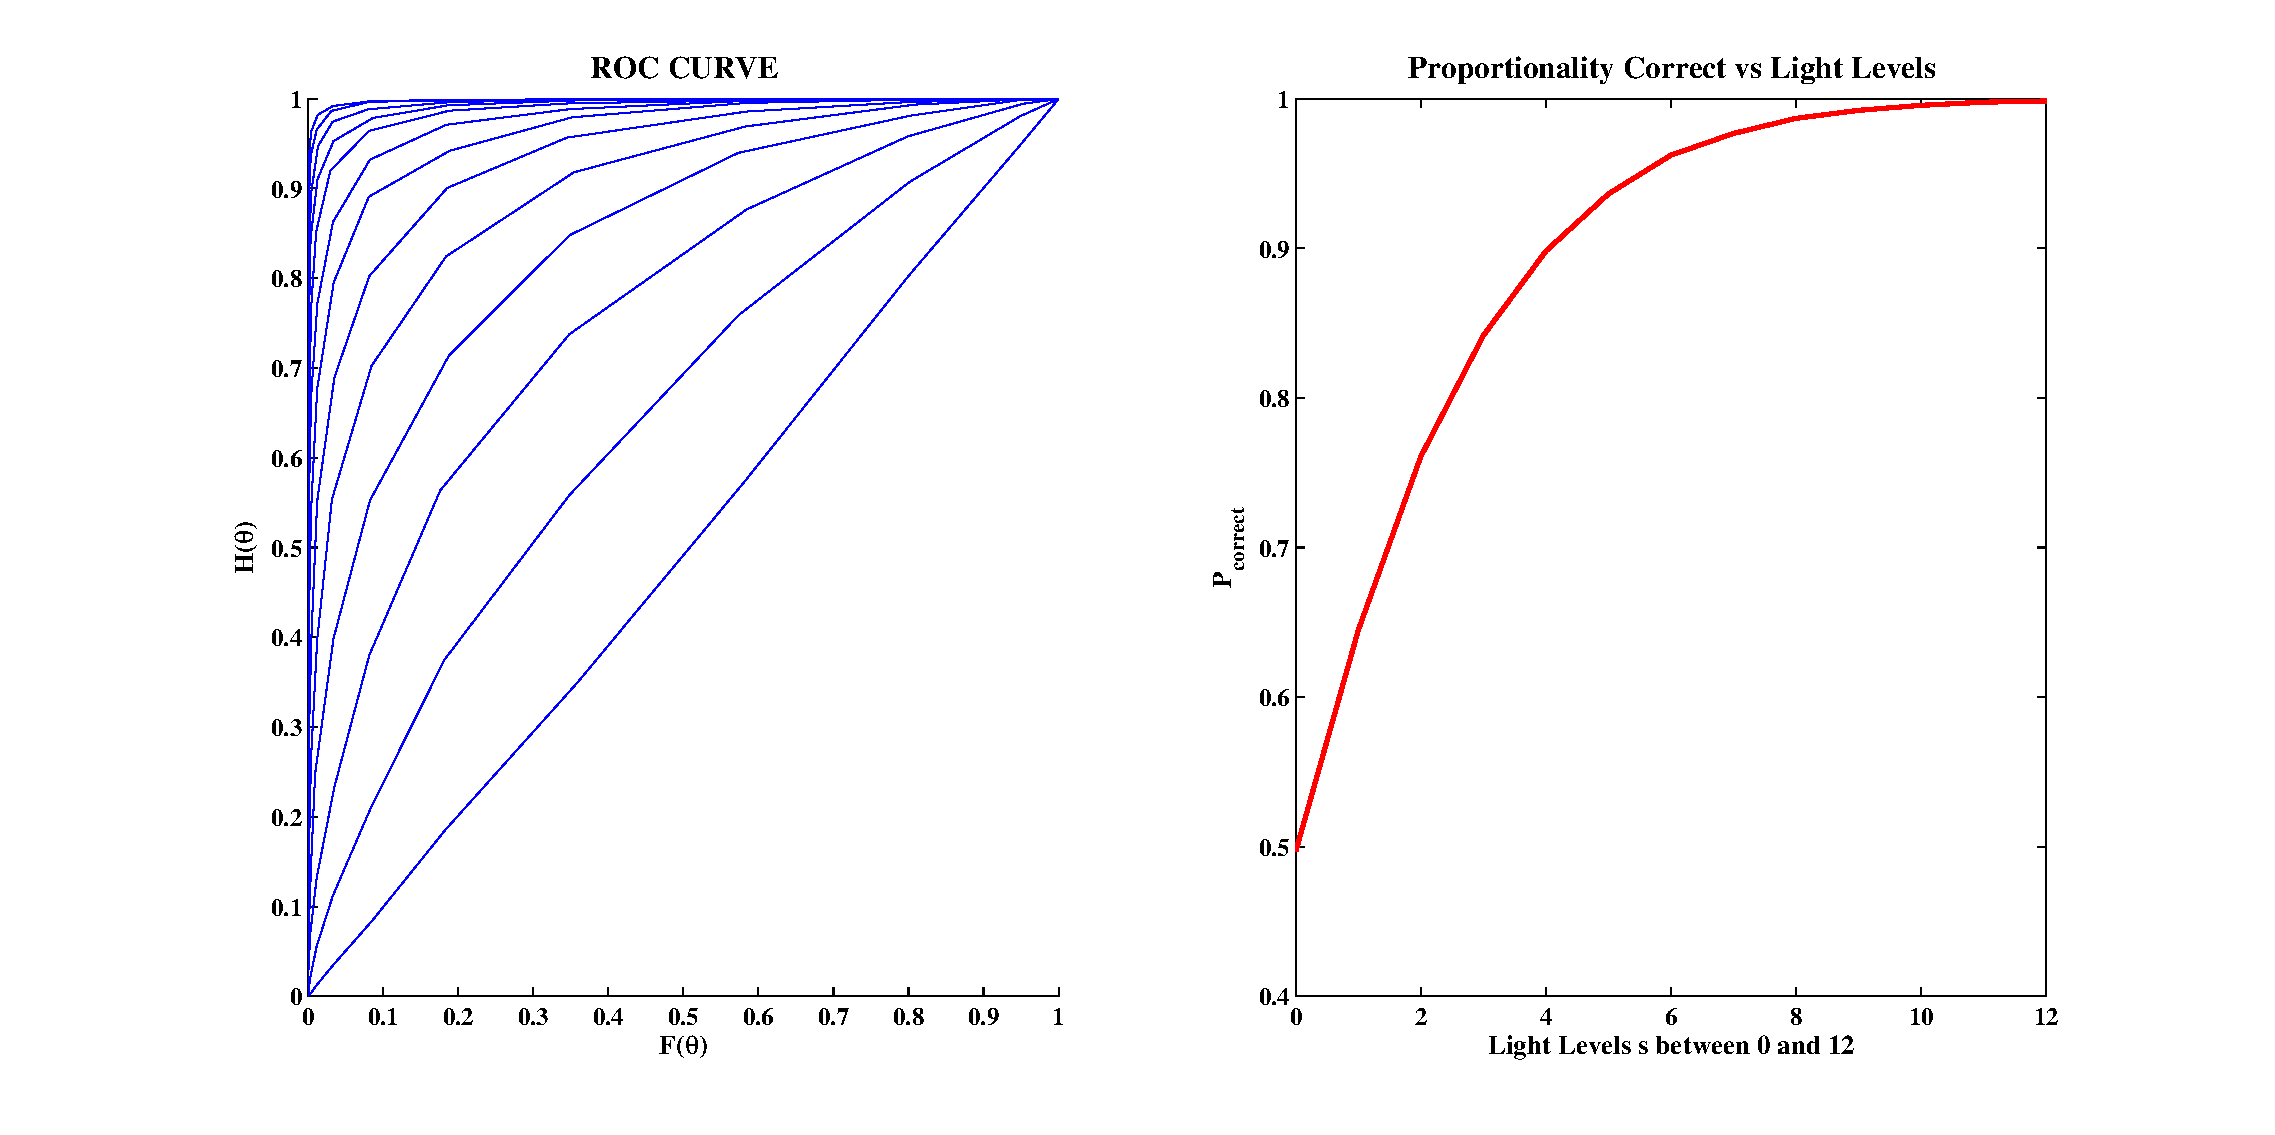
\includegraphics[width=\textwidth]{roc.eps}
\begin{footnotesize} Fig. 5, Each curve on the ROC CURVE graph is eliminated by using $\theta=0:1:31$, and each curve stands for one specific light level \textit{s}. There exists 13 curves because $s=0:1:12$.The area under each curve is computed by \textbf{trapz} command on MATLAB. Each area corresponds to $P_{correct}$. The right graph shows $P_{correct}$ for each light level.  
\end{footnotesize}
\end{center}











\end{document}